\sep
\Satz[3.1 Wahrscheinlichkeit eines Punktes] \newline
Sei \( X : \omega \rightarrow \R \) eine Zufallsvariable mit Verteilungsfunktion F. Für jdedes a in \(\R\) gilt \[ \mathbb{P}[X = a] = F(a) - F(-a)\]
\Def[3.2] \newline
Sei \( A \in \mathcal{F} \) ein Ereignis. Wir sagen A tritt fast sicher ein falls \[ \mathbb{P}[A] = 1\]
\Def[3.4 Diskrete Zufallsvariable] \newline
Eine Zufallsvariable \( X : \omega \rightarrow \R \) hiest diskret falls eine endliche oder abzählbare Menge \( W \subset \R\) existiert, sodass \[ \mathbb{P}[X \in W ] = 1\]
\Bem[3.5] Wenn der Grundraum \( \omega\) endlich oder abzähbar ist, dann ist jede Zufallsvariable \( X : \omega \rightarrow \R\) diskret.
\Def[3.6 Verteilung von X] \newline
Sei X eine diskrete Zufallsvariable mit Werten in einer endlichen oder abzähbaren Menge \( W \subset \R\). Die Zahlenfolge \((p(x))_{x \in W}\) definiert durch \[ \forall x \in W \ p(x) := \mathbb{P}[X = x]\] heisst Verteilung von X
\Satz[3.7] Die Verteilung \((p(x))_{x \in W}\) einer diskreten Zufallsvariable erfüllt \[ \sum_{x \in W} p(x) = 1\]
\Satz[3.9] Sei X eine diskrete Zufallsvariable, dessen WErte in einer endlichen oder abzähbaren Menge W liegen, und deren Verteilung p ist. Dann ist die Verteilungsfunktion von X gegeben durch \[ \forall X \in \R \ F_X(x) = \sum_{y \leq x_{y \in W}}p(y)\]
\Def[3.10 Bernoulli Verteilung] \newline
Es sei \( 0 \leq p \leq 1\). Eine Zufallsvariable X heisst Bernoulli Zufallsvariable mit Parameter p, wenn sie Werte in W \( = \{0,1\}\) annimt und folgendes gilt \[ \mathbb{P}[X=0] = 1-p \quad \text{und} \ \mathbb{P}[X=1] = p\]
\Def[3.11 Binomialverteilung] \newline
Sei \( 0 \leq p \leq 1\), sein \( n \in \N\). Eine Zufallsvariable X heisst binomiale Zufallsvariable mit Paramtern n und p, wenn sie werte in \( W = \{ 0, \dots , n\}\) annimt und folgendes gilt \[\forall k \in \{0, \dots , n\} \ \mathbb{P}[X=k] = \binom{n}{k} p^k(1-p)^{n-k}\]
\Satz[3.13 Sum von unab. Bern. und Binom. Z.V] \newline
Sei \( 0 \leq p \leq 1\), sein \( n \in \N\). Seien \( X_1, \dots, X_n\) unabhängige Bernoulli Z.V mit Parameter p. Dann ist \[ S_n := X_1 + \dots + X_n\] eine binomialverteilte Z.V mit paramtern n und p.
\Bem[3.14] \newline
Bin(1,p) ist gerade Ber(p) verteilt. Falls \(X \sim Bin(m,p), Y \sim Bin(n,p) \) und X,Y unabhängig, dann ist \(X + Y \sim Bin(m+n, p)\)  verteilt.
\Def[3.15 Geometrische Verteilung] \newline
Es sei \( 0 < p \leq 1\). Eine Zufallsvariable X heisst geometrische Zufallsvariable mit Parameter p, falls sie Werte in W = \( \N \setminus \{0\}\) annimt und folgendes gilt \[\forall k \in \N \setminus \{0\} \ \mathbb{P}[X=k] = (1-p)^{k-1} \cdot p\]
\Bem[3.16] \newline
Für p=1 und k = 1 erscheint in der obigen Gleichung \(0^0 = 1\) , es gilt \( \mathbb{P}[X=1] = p\)
\Satz[3.18] \newline
Sei \(X_1, X_2, \dots \) eine Folge von unendlich vielen unabhängigen Bernoulli Z.V mit Parameter p. Dann ist \[ T:= \min\{n \geq 1 : X_n = 1\}\] eine geometrisch verteilte Zufallsvariable mit Paramter p.
\Bem[3.18A] \newline
Sei T eine geometrische Verteilung mit Parameter p. Dann ist \( T > n\), wenn die ersten n Bernoulli-Experimente fehlschlagen. Daher gilt \[ \mathbb{P}[T > n] = (1-p)^n\]
\Satz[3.20 Gedächnislosigkeit der Geo. Vert.] \newline
Sei \( T \sim Geom(p)\) für \( 0 < p < 1\). Dann gilt \[ \forall n \geq 0 \quad \forall k \geq 1 \quad \mathbb{P}[T \geq n + k | T > n] = P[T \geq k]\]
\Def[3.21] \newline
Sei \( \lambda > 0\) eine positive reelle Zahl. Eine Zufallsvariable X heisst Poisson-Zufallsvariable mit Paramter \( \lambda\), wenn sie Werte in \( W = \N \) annimt und folgendes gilt \[ \forall k \in \N \ \mathbb{P}[X = k] = \frac{\lambda^k}{k!}\exp^{-\lambda}\]
\Satz[3.23 Poisson-Approx. der Binom. verteil.] \newline
Sei \( \lambda > 0\). Für jedes \( n \geq 1 \) seien \( X_n \sim Bin(n, \frac{\lambda}{n})\)  Zufallsvariablen. Dann gilt \[ \forall k \in \N \ \lim_{n \rightarrow \infty } \mathbb{P}[X_n = k] = \mathbb{P}[N =k]\]
\Def[3.25 Stetig verteilte Zufallsvariablen] \newline
Eine Zufallsvariable \( X: \omega \rightarrow \R \) heisst stetig, wenn ihre Verteilungsfunktion \(F_X \) wie folgt geschrieben werden kann \[F_X(a) = \int_{-\infty}^{a} f(x)dx \ \text{für alle a in} \ \R\] wobei \(f: \R \rightarrow \R_+\) eine nicht-negative Funktion ist. Wir nennen dann f Dichte von X. Weiter gilt für f \[1 = \int_{-\infty}^{\infty} f(x) dx\] \newline
\Bem[3.25A] \newline
\(f(x)dx \) ist die Wahrscheinlichkeit, dass X Werte in \( [x, x+ dx]\) annimmt. Die Stetigkeit von \(F_X \)folgt dabei aus der Definition (3.25). Ausserdem folgt aus Satz 3.1, dass \[ \forall x \in \R  \ \mathbb{P}[X = x] = 0\]Die Wahrscheinlichkeit für das Auftreten jedes einzelnen Werts der Zufallsvariablen beträgt exakt Null\newline
\Bem[3.25B] \newline
Von f zu \( F_X\) : Sei X eine stetige Z.V und f die Dichte. \(F_X\) können wir mit \[F_X(x) = \int_{-\infty}^x f(y)dy\]. Es liegt nahe, dass wir die Dichte mittels Ableiten herausfinden. \newline
\Theo[3.26] \newline
Sei X eine Zufallsvariable. Die Verteilungsfunktion \(F_X\) sei stetig und Stückweise \( C^1\), d.h es gibt \(x_0 = -\infty < x_1 < \dots < x_{n-1} < x_n = + \infty\), sodass \(F_X\) auf jedem Intervall \( (x_i, x_{i+1})\) Element von \(C^1\) ist. Dann ist X eine stetige Zufallsvariable und die Dichte f kann konstruiert werden, indem man folgendes festlegt \[ \forall x \in (x_i, x_{i+1}) \ f(x) = F'_X(x)\]
\Def[3.27 Gleichverteilung auf [a,b]] \newline
Eine stetige Zufallsvariable X heisst gleichverteilt auf \([a,b]\) falls ihre Dichte gegeben ist durch \[ f_{a,b}(x) = \begin{cases}
    \frac{1}{b-a} & x \in [a,b] \\
    0 & x \notin [a,b]
\end{cases}\]
Wir schreiben \(X \sim \mathcal{U}([a,b])\) \newline
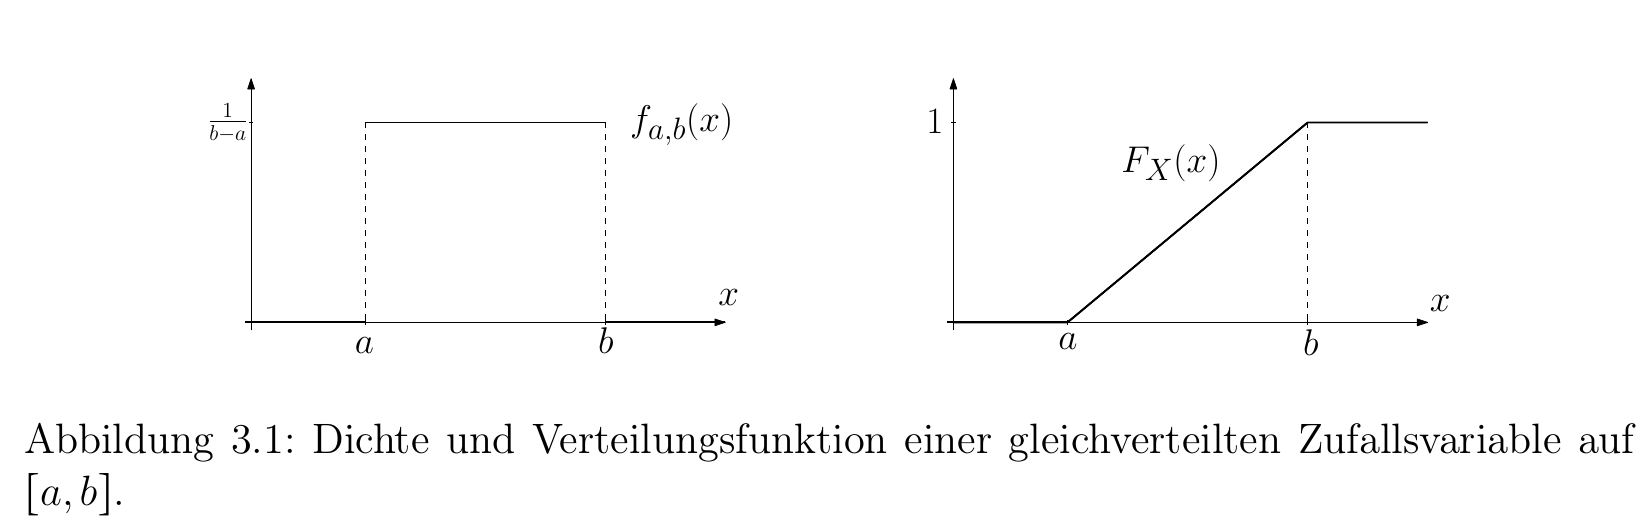
\includegraphics[scale=0.1]{Gleichverteilt.png}
\Bem[3.27A]
\begin{itemize}
    \item Die Wahrscheinlichkeit in einem Interval \( [c, c + \ell] \subset [a,b]\) zu fallen ist lediglich abhängig von dessen Länge \( \ell\) \[\mathbb{P}[X \in [c, c + \ell ]] = \frac{\ell}{b-a}\]
    \item Die Verteilungsfunktion X ist gegeben durch \[ F_X(x) = \begin{cases}
        0 & x < a \\
        \frac{x-a}{b-a} & a \leq x \leq b \\
        1 & x > b
    \end{cases}\]
\end{itemize}
\Def[3.28 Exponentialverteilung mit \(\lambda > 0\) ] \newline
Eine stetige Zufallsvariable T heisst exponentialverteilt mit Parameter \( \lambda > 0\) falls ihre Dichte gegeben ist durch
\[ f_\lambda(x) = \begin{cases}
    \lambda \exp ^{-\lambda x } & x \geq 0 \\
    0 & x < 0
\end{cases}\]
\Bem[3.28A]
Die Grafik zeigt die Dichte und Verteilungsfunktion einer exponentialverteilten Zufallsvariable mit Parameter \( \lambda\)
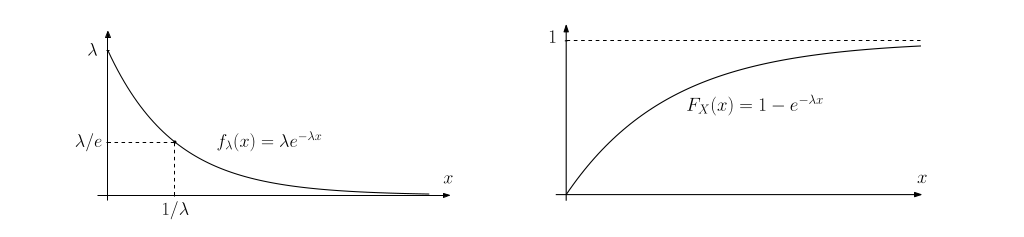
\includegraphics[scale=0.2]{exp_Dichte_Verteilung.png} \\ 
T modelliert häufig die Lebensdauer oder Wartezeit eines allgemeinen Ergebnisses. \\
Eigenschaften: \begin{itemize}
    \item Die Wahrscheinlichkeit des Wartens ist exponentiell klein: \[ \forall t \geq 0 \ \mathbb{P}[T > t] = \exp^{-\lambda t }\]
    \item T besitzt die Eigenschaft der Gedächnislosigkeit \[ \forall t,s > 0 \ \mathbb{P}[T > t + s | T > t] = [T > s]\]
\end{itemize}
\Def[3.29] \newline
Eine stetige Zufallsvariable X heisst normal verteilt mit Parametern m und \( \sigma^2 > 0\) falls ihre Dichte gegeben ist durch \[ f_{m,\sigma}(x) = \frac{1}{\sqrt{2 \pi \sigma^2}}\exp^{-\frac{(x-m)^2}{2 \sigma^2}}\]
Wir schreiben \( X \sim \mathcal{N}(m, \sigma^2)\) \newline
\Bem[3.29A] \newline
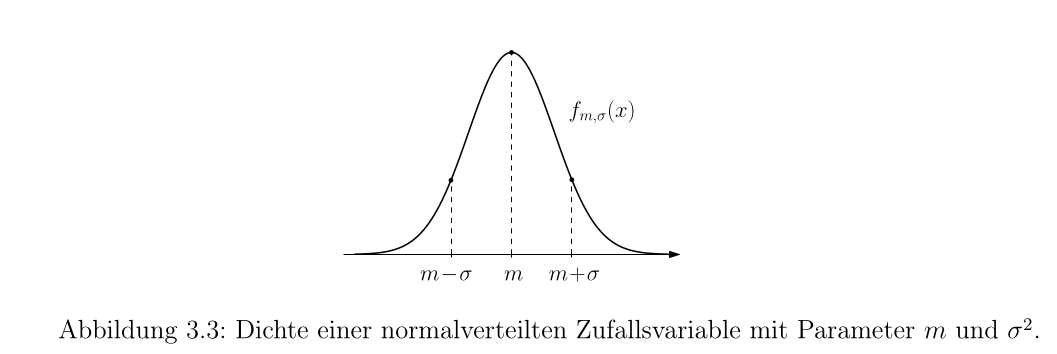
\includegraphics[scale=0.175]{Dichte_Normalverteilung.png} \\
Zum Beispiel bei einer physikalischen Messung kann der parameter \( \sigma\) die Schwankung von X darstellen und generell zeigt ein kleines \(\sigma\) eine genaue Messung an und ein grosses \(\sigma\) eine ungenaue.
Eigenschaften : \begin{itemize}
    \item Seien \(X_1, \dots X_n\) unabhängige normalverteilte Zufallsvariablen mit Parametern \((m_1, \sigma_1^2), \dots , (m_n, \sigma_n^2)\) dann ist \[ Z = m_0 + \lambda_1 X_1 + \dots + \lambda_n X_n \] eine normalverteilte Zufallsvariable mit Parametern \(m = m_0 + \lambda_1 m_1 + \dots + \lambda_n m_n\) und \(\sigma^2 = \lambda_1^2 \sigma_1^2 + \dots + \lambda_n^2 \sigma_n^2\)
    \item Wir sprechen im Fall von  \( X \sim \mathcal{N}(0,1)\), gerade von einer standardnormalverteilten Zufallsvariable. Man merke sich dann folgende Beziehung \[ Z = m + \lambda \cdot X\], wobei X eine normalverteilte Zufallsvariable mit Parametern m und \(\sigma^2\) ist.
    \item Falls X normalverteilt mit Parametern m und \( \sigma^2 \) ist, dann liegt die "meiste " Wahrscheinlichkeitsmasse der Z.V im Intervall \( [m - 3\sigma, m + 3\sigma ]\). Es gilt gerade \[ \mathbb{P}[\abs{X - m} \geq 3 \sigma ] \leq 0.0027\]
\end{itemize}

